\subsubsection*{Obteniendo el valor máximo}
 El problema de la mochila analiza, para cada objeto, el máximo valor que se puede obtener para cada capacidad posible de la mochila. Si llamamos $K$ a la capacidad de la mochila, se evaluará introducir un elemento $e$ en la capacidad $k$ con 1 $\leq$ $k$ $\leq$ $K$. 

En cada evaluación se decide entre no meter el elemento, con lo cual el valor máximo de la mochila que tenga la capacidad $k$ será el calculado con algún elemento anterior (o cero en el caso de que sea el primero en ser evaluado); o meter el elemento, con lo cual, al valor del elemento se le suma el valor de la mochila de capacidad k - $peso(e)$ que sea máxima. De esta forma, se genera un subproblema que respeta el principio de optimalidad, con lo cual se puede aplicar programación dinámica para solucionar el problema. \\
 
  Extendiendonos a 2 mochilas, al evaluar la $k$ posibilidad de la primer mochila (con capacidad $K_{a}$), se debe tener en cuenta que tambien está la posibilidad de utilizar la segunda mochila (con capacidad $K_{b}$). Esto nos muestra que por cada elemento debemos calcular $K_{a} \times K_{b}$ combinaciones de capacidades. Sin contar el primer elemento, el resto calculará sus combinaciones en base a las del elemento que le precedió en la evaluación, siguiendo la idea del algoritmo original de una mochila. Para obtener el valor final, se buscará en la matriz resultante de evaluar el último elemento, a la combinación de capacidades entre ambas mochilas que resulte máxima.\\
  
  \vspace*{0.3cm} \vspace*{0.3cm}
  \begin{center}
 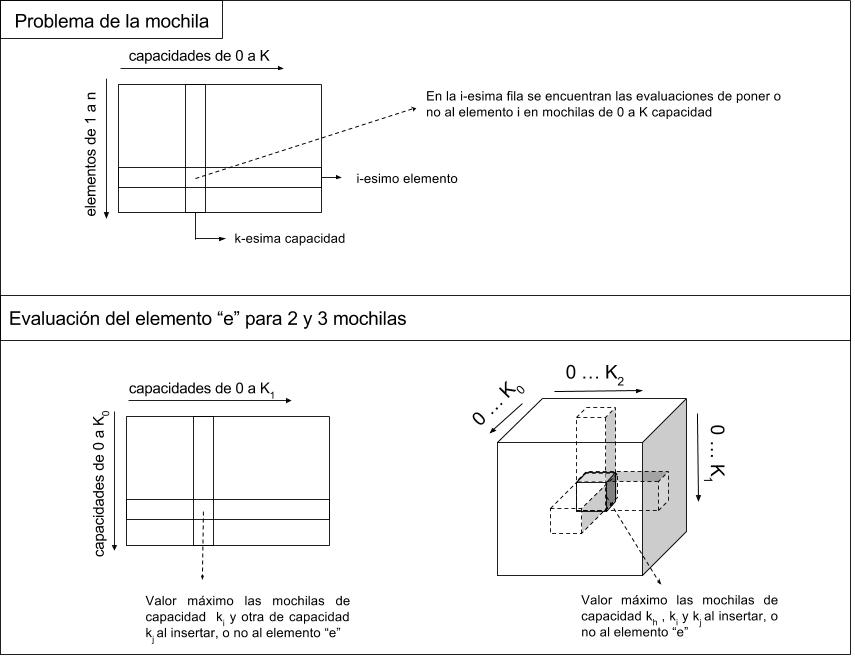
\includegraphics[scale=0.6]{./EJ3/dibujo-matrices.jpg}
  \end{center}
  \vspace*{0.3cm}
  
  Con la misma lógica podemos ver que para 3 mochilas donde se tienen capacidades  $K_{a}$,$K_{b}$ y $K_{c}$, cada elemento disponible evaluará $K_{a} \times K_{b} \times K_{c}$ posibilidades. En este caso se buscará la solución en la matriz tridimensionál de posibilidades obtenidas del último elemento evaluado.

\subsubsection*{Recuperando los elementos utilizados}

Siendo que la consigna pide los objetos involucrados en la solución, es necesaria una forma de, a partir de los valores máximos obtenidos, deducir los elementos que fueron usados y el lugar donde fueron colocados para lograr el resultado.\\

Analizando la última matriz del caso de 2 mochilas (sin perder generalización para 3 mochilas), podemos notar que por cada objeto que iteramos para intentar encontrarle un lugar en las mochilas, deja el valor previo, de cada combinacion de capacidades, sin tocar cuando el objeto no es utilizado. Al ser utilizado, se cambia el valor por el nuevo máximo alcanzado. De utilizar 1 matriz solamente, y actualizarla por cada objeto, se perderá la posibilidad de saber si se usó o no a cada uno, ya que no se tendrá un "paso anterior" por haber sido reescrito en cada paso subsiguiente. \\

Para recuperar estos estados, se resuelve guardar la matriz involucrada en el c\'alculo de cada elemento. Llamando a las matrices del elemento i M, y N a la del elemento j subsiguiente a i (ambas de dimensión $K_{a} \times K_{b}$), se tiene que si el maximo se encuentra en $N_{yz}$ y es igual a $M_{yz}$, entonces quiere decir que el algoritmo al evaluar la posibilidad de meter al elemento j en esa combinación, opto por excluirlo, con lo cual no es perteneciente a la solución final. Si en cambio el valor es superior, indica que el valor guardado en la instancia M fue incrementado, y usado a j en la solución.\\

Finalmente, para saber en que mochila fue introducido cada elemento, se busca en la instancia M, mochila a cuya capacidad se le restó el peso $p(j)$ de j. Esto lo podemos saber cuando el valor de $N_{yz} = M_{(y-p(j),z)}$ en el caso de que se encuentre en la mochila "a" o $N_{yz} = M_{(y,z-p(j))}$ en caso contrario.\\

  \vspace*{0.3cm} \vspace*{0.3cm}
  \begin{center}
 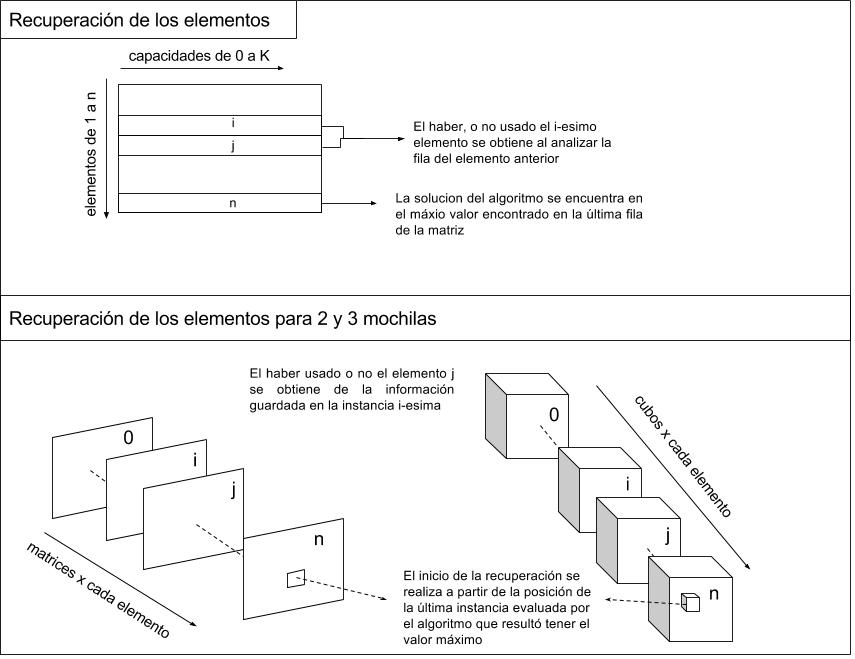
\includegraphics[scale=0.6]{./EJ3/dibujo-recuperacion.jpg}
  \end{center}
  \vspace*{0.3cm}

 Para el caso de 3 mochilas, no se pierde generalidad: En vez de contar con matrices bidimensionales se utilizan tridimensionales, y se compara $N_{xyz} = M_{(x-p(j),y,z)}$, $N_{xyz} = M_{(x,y-p(j),z)}$, $N_{xyz} = M_{(x,y,z-p(j))}$ para determinar la pertenencia de cada objeto a la solución.     